\documentclass[hyperref, UTF8]{ctexart}
\usepackage{graphicx}
\usepackage{float}
\usepackage{amsmath}
\usepackage{amsfonts}
\usepackage{amssymb}
\usepackage{fontspec}
\usepackage{tikz}
\setmonofont{Consolas}
\setCJKmainfont{Noto Sans S Chinese Regular}
\usetikzlibrary{shapes.geometric, arrows}
\tikzstyle{startstop} = [rectangle, rounded corners, minimum width=3cm, minimum height=1cm,text centered, draw=black, fill=red!30]
\tikzstyle{io} = [trapezium, trapezium left angle=70, trapezium right angle=110, minimum width=3cm, minimum height=1cm, text centered, draw=black, fill=blue!30]
\tikzstyle{process} = [rectangle, minimum width=3cm, minimum height=1cm, text centered, draw=black, fill=orange!30]
\tikzstyle{decision} = [diamond, minimum width=3cm, minimum height=1cm, text centered, draw=black, fill=green!30]
\tikzstyle{arrow} = [thick,->,>=stealth]
\usepackage[a4paper, top=3cm, bottom=3cm, left=3cm, right=3cm]{geometry}
\usepackage{subcaption}
\usepackage{xcolor}
\usepackage{animate}
\usepackage{listings}
\lstset{
	keywordstyle=\color{blue!70},
	commentstyle=\color{red!50!green!50!blue!50},
	frame=shadowbox,
	rulesepcolor=\color{red!20!green!20!blue!20},
	tabsize=2,
	basicstyle=\ttfamily\small,
	numberstyle=\tiny,
	numbers=left,
	showstringspaces=false,
	breaklines=true,
	language=MATLAB
}
\hypersetup{
	colorlinks=true,
	bookmarks=true,
	bookmarksopen=true,
	pdftitle=遥感综合实验~遥感图像分类实验报告,
	pdfauthor=16020710017~蓝彧文,
	linkcolor=blue
}
\title{遥感综合实验实验报告\\遥感图像分类}
\author{蓝彧文~16020710017}
\begin{document}
	\maketitle
	\tableofcontents
	\newpage
	实验中使用的所有代码和数据可以在\\ \url{https://github.com/EwenLan/remote-sensing-library}获取。
	\section{实验四~无监督分类}
	\subsection{实验目的}
理解遥感图像分类的概念,掌握一些典型的图像无监督分类方法,例如K均值聚类算法。完成遥感图像的图像分类。
\subsection{实验原理}
\begin{figure}[H]
	\centering
	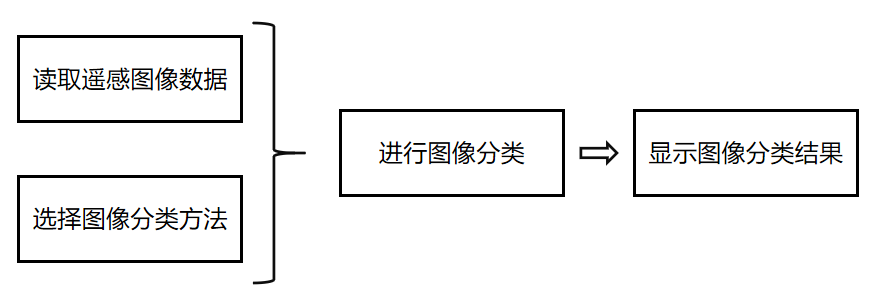
\includegraphics[width=0.7\linewidth]{figure/classification_flowchart.png}
	\caption{进行图像分类的步骤}
\end{figure}
\subsubsection{图像分类的概念}
将图像中的像素点划分为不同的类别,每一个类别具有特定的物理含义。例如不同的地物类型,包括草地、水泥地、建筑、道路、森林、山地等。

图像分类的两个步骤:特征提取和分类算法。
\begin{description}
	\item[特征提取] 如何描述每一个像素点,颜色特征向量。
	\item[分类算法] k均值据类算法。
\end{description}
\subsubsection{k均值聚类算法}
k均值据类算法是一个迭代算法,迭代更新每一个类别的聚类中心,并且通过最近邻准则完成分类。
\begin{description}
	\item[算法描述] \begin{enumerate}
		\item 任选K个初始聚类中心:$Z_1(1)$,$Z_2(1)$,$\dots$,$Z_K(1)$
		\item 按最小距离原则叫其余样本分配到K各聚类中心中的某一个,即
		\[ \text{若} \min\left\lbrace \left\| \mathbf{X}-\mathbf{Z}_i(k) \right\|,i=1,2,\dots,K \right\rbrace=\left\| \mathbf{X}-\mathbf{Z}_j(k) \right\|=D_j(k) \]
		则$X\in S_j(k)$
		\item  计算各个聚类中心的新向量值:$\mathbf{Z}_j(k+1)\quad j=1,2,\dots,K$
		\[ \mathbf{Z}_j(k+1)=\frac{1}{N_j}\sum_{\mathbf{X}\in S_j(k)}\mathbf{X}\quad j=1,2,\dots,K \]
		\item 如果$\mathbf{Z}_j(k+1)\neq\mathbf{Z}_j(k)\quad j=1,2,\dots,K$,则回到2,将模式样本逐个重新分类,重复迭代计算。
		\item 如果$\mathbf{Z}_j(k+1)=\mathbf{Z}_j(k)\quad j=1,2,\dots,K$,算法收敛,计算完毕。
	\end{enumerate} 
\end{description}
\subsection{实验流程}
\begin{figure}[H]
	\centering
	\begin{tikzpicture}[node distance=1.5cm]
	\node(start) [startstop] {开始};
	\node(input_img) [io, below of=start] {输入待分类的图像};
	\node(random_center) [process, below of=input_img] {随机选取聚类中心};
	\node(calculate_distance) [process, below of=random_center] {计算所有像素到每一个聚类点的距离};
	\node(classifing) [process, below of=calculate_distance] {根据距离对像素点归类};
	\node(convergent) [decision, below of=classifing, yshift=-1.5cm] {算法是否收敛?};
	\node(calculate_center) [process, right of=convergent, xshift=3cm] {重新计算聚类点的坐标};
	\node(display) [io, below of=convergent, yshift=-1.5cm] {显示聚类结果};
	\node(end) [startstop, below of=display] {结束};
	
	\draw[arrow] (start) -- (input_img);
	\draw[arrow] (input_img) -- (random_center);
	\draw[arrow] (random_center) -- (calculate_distance);
	\draw[arrow] (calculate_distance) -- (classifing);
	\draw[arrow] (classifing) -- (convergent);
	\draw[arrow] (convergent) -- node[anchor=east] {是} (display);
	\draw[arrow] (convergent) -- node[anchor=south] {否} (calculate_center);
	\draw[arrow] (calculate_center) |- (calculate_distance);
	\draw[arrow] (display) -- (end);
	\end{tikzpicture}
\end{figure}
\subsection{实验程序}
\lstinputlisting[caption={K均值聚类程序}]{"../Executable Script/Exp 4/ReadAirportImages.m"}
\subsection{实验结果和分析}
对如图\ref{fig:airport_44}所示的图片上的像素进行聚类。设置聚类数为$2$,初始聚类中心设置为随机数,可以得到如图\ref{fig:airport_44_class_1_logical}和图\ref{fig:airport_44_class_2_logical}所示的分类结果。
\begin{figure}[H]
	\centering
	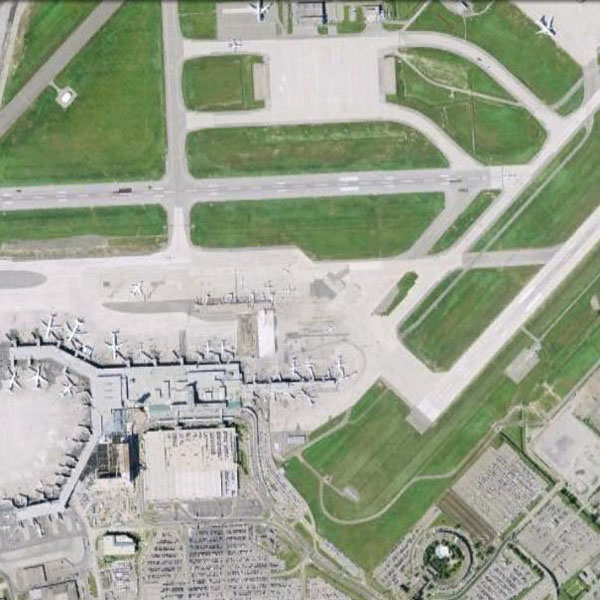
\includegraphics[width=0.7\linewidth]{figure/airport_44.jpg}
	\caption{飞机场原图}
	\label{fig:airport_44}
\end{figure}
\begin{figure}[H]
	\centering
	\begin{minipage}{0.45\linewidth}
		\centering
		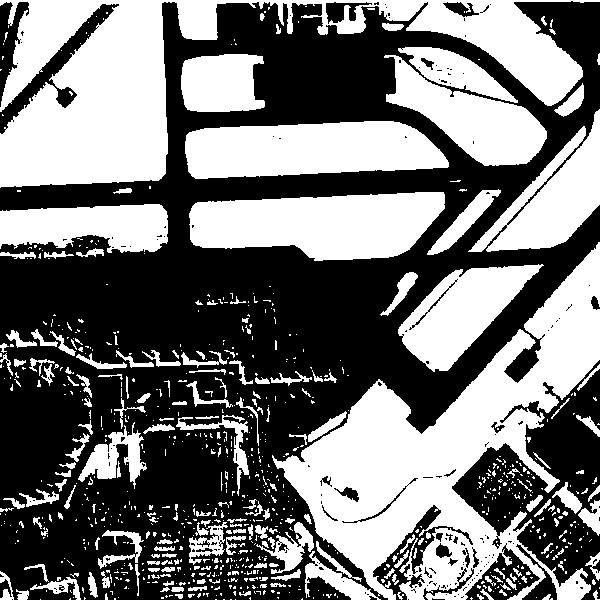
\includegraphics[width=\linewidth]{figure/airport_44_Class_01_Logical.png}
		\caption{第一个分类的分类图}
		\label{fig:airport_44_class_1_logical}
	\end{minipage}
	\begin{minipage}{0.45\linewidth}
		\centering
		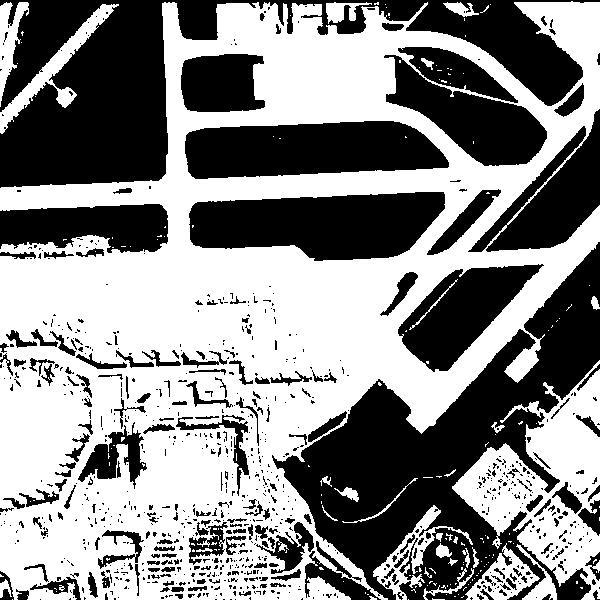
\includegraphics[width=\linewidth]{figure/airport_44_Class_02_Logical.png}
		\caption{第二个分类的分类图}
		\label{fig:airport_44_class_2_logical}
	\end{minipage}
\end{figure}
其中,逻辑分类图中的白色区域代表图片中这个区域的像素点属于这一个分类。如果将原图片中的分类结果提取,可以得到如图\ref{fig:airport_44_class_1_separated}和图\ref{fig:airport_44_class_2_separated}所示的结果。
\begin{figure}[H]
	\centering
	\begin{minipage}{0.45\linewidth}
		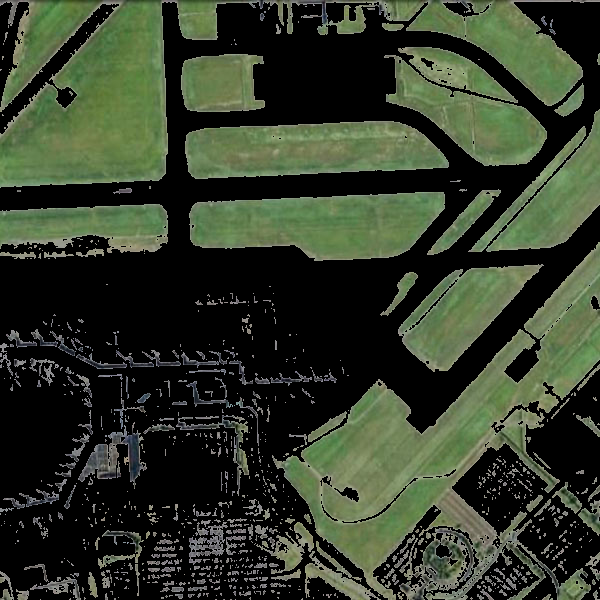
\includegraphics[width=\linewidth]{figure/airport_44_Class_01_Separated.png}
		\caption{分类一在原图片上的内容}
		\label{fig:airport_44_class_1_separated}
	\end{minipage}
	\begin{minipage}{0.45\linewidth}
		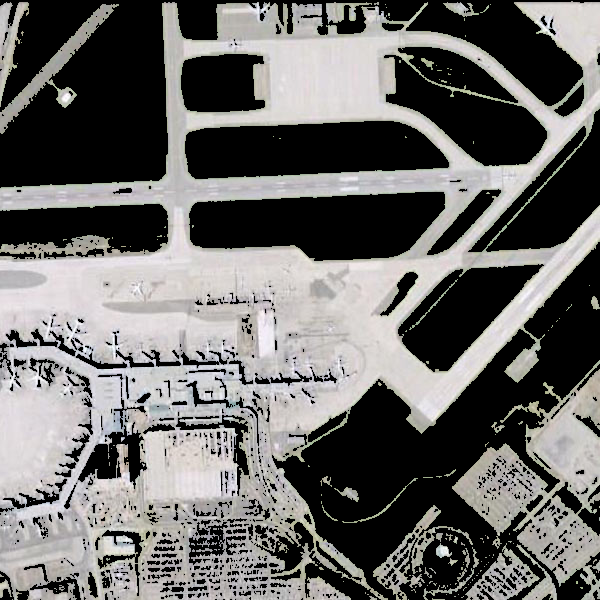
\includegraphics[width=\linewidth]{figure/airport_44_Class_02_Separated.png}
		\caption{分类二在原图片上的内容}
		\label{fig:airport_44_class_2_separated}
	\end{minipage}
\end{figure}
将k均值无监督分类过程进行统计分析,可以绘制如图\ref{fig:airport_44_animate}所示的图表\footnote{动画演示。如果不能播放可以尝试更换pdf阅读器,例如:Adobe Acrobat Reader。}。
\begin{figure}[H]
	\centering
	\animategraphics[autopause, autoresume, loop, autoplay, width=0.7\linewidth]{5}{figure/airport_44_Clustering_Latex_Animate/frame-}{0001}{0010}
	\caption{聚类点位置和分类过程(动画)}
	\label{fig:airport_44_animate}
\end{figure}
可以看到,在训练过程中,各像素点的分类会逐步收敛,最终达到稳定,形成最佳的分类结果。
\end{document}